%!TEX root = ../dissertation.tex

\graphicspath{{5-pilot/figures/}}
\chapter{Pilot Studies}
\label{ch:pilot}


This chapter provides some preliminary results of the two ongoing projects toward the direction of the thesis. While not directly being a part of the overall system as described in Figure \ref{fig:grand}, these experiments are expected to provide valuable insights about what convolutional neural network and deep generative models can learn from music audio signals, and how their architecture should be designed to maximize the effectiveness.

\section{Pitch Estimation using Time-Domain Convolutional Neural Network}

The first project concerns the problem of monophonic pitch estimation.
To date the best performing techniques, such as the pYIN algorithm \cite{mauch2014pyin}, are based on a combination of DSP pipelines and heuristics.
While such techniques perform very well on average, there remain many cases in which they fail to correctly estimate the pitch or determine when a pitched sound is present.
For example, pYIN algorithms are relatively accurate for male and female singing voices, but the accuracy drops to near 0 for piccolo flute sounds.
This motivates a data-driven approach for pitch estimation, where the model can learn different methods to estimate the pitch depending on the individual instrument or timbre.

\begin{figure}
	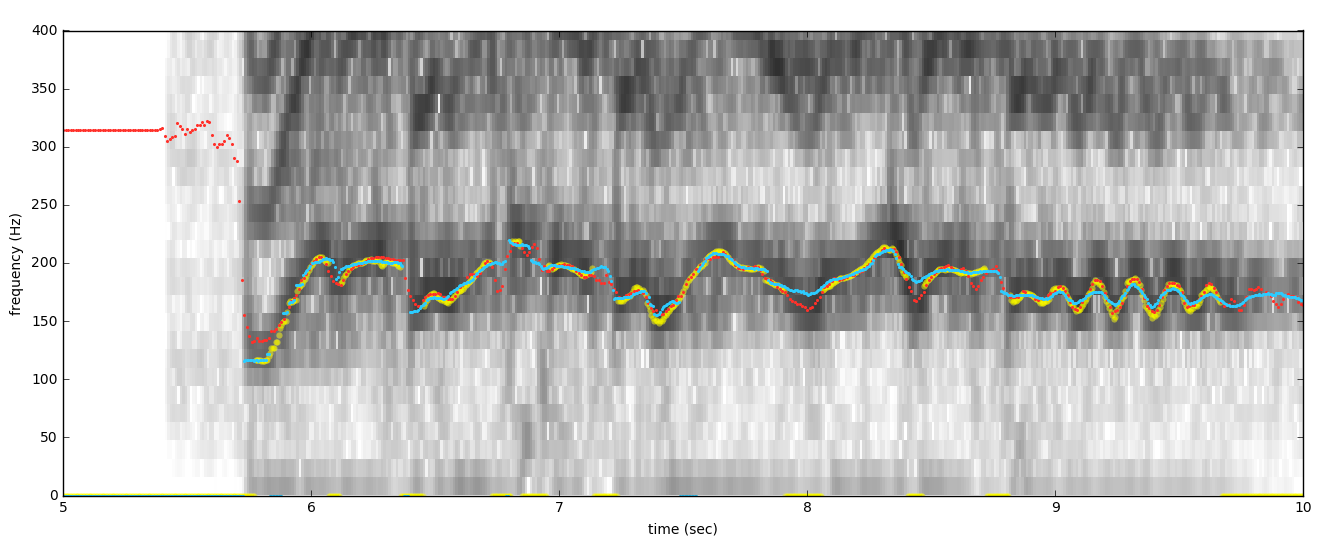
\includegraphics[width=\textwidth]{crepe.png}
	\caption{Frequency estimation as produced by pYIN (cyan) and the proposed time-domain convolutional neural network (red), superimposed over the ground truth (yellow) and the spectrogram. CNN performs close to pYIN without any temporal processing.}\label{fig:crepe}
\end{figure}

Using a deep convolutional neural network with 6 convolutional layers with batch normalizations, ReLU activations, and dropouts, the model could achieve comparable but yet slightly lower raw pitch accuracy (90.3\%) than pYIN (94.6\%) on a subset of MedleyDB \cite{bittner2014medleydb} melodies.
The resulting pitch traces of CNN and pYIN is shown in Figure \ref{fig:crepe}.
Unlike pYIN, no postprocessing operations for temporal smoothing is applied in the CNN result.
It suggests that a better performance should be achievable, using more sophisticated models such as convolutional recurrent neural network (CRNN) or dilated convolutions and training from more diverse training dataset.


\section{Generative Adversarial Network of Orchestral Instrument Sounds}

As seen in Section \ref{sec:deeplearning}, the recent surge of GAN variants have shown many promising results in computer vision.
To examine the potential applicability of a GAN model in music, a few attempts were made to train GANs that learns from musical sounds, in the form of raw audio waveforms and magnitude spectrograms.
A difference between audio and images is that audio has much more high-dimensional data than the typical images used in deep learning.
Time domain signals have tens of thousands of numbers for a second of audio, and a typical resolution of a magnitude spectrogram ranges from 512 to 1024 vertical pixels where many image datasets for deep learning is under 96 pixels.
Despite this difficulty, a careful design using mode regularized generative adversarial network (MRGAN) \cite{che2016mrgan} could achieve a stable convergence of 512-by-64 images of magnitude spectrograms, as shown in Figure \ref{fig:gan}.

\begin{figure}
	\centering
	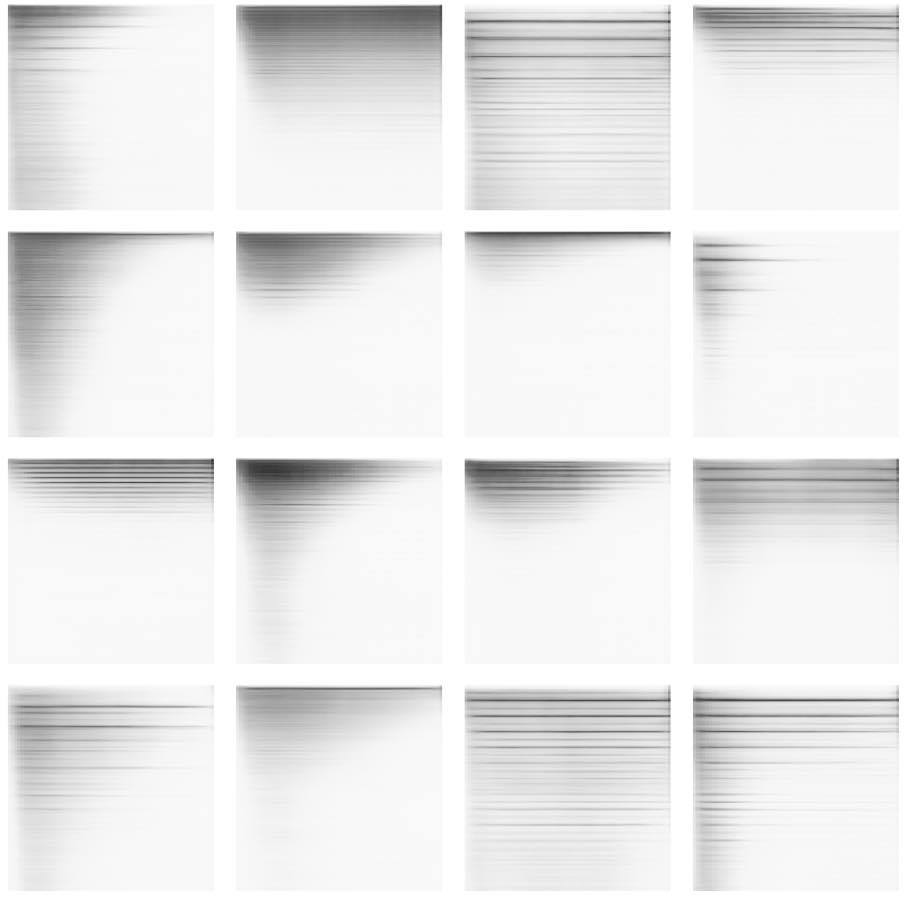
\includegraphics[width=0.55\textwidth]{gan.jpg}
	\caption{Spectrogram images generated by mode regularized generative adversarial network (MRGAN) %\cite{che2016mrgan} trained on instrumental sounds of Vienna symphonic library
	}\label{fig:gan}
\end{figure}

Future work in this project includes quantifying how the manifold learned by the GAN is informative in predicting various qualities of the sound, by combining the model with other GAN variants like InfoGAN \cite{chen2016infogan} or ACGAN \cite{odena2016acgan}.
Using NSynth dataset will also help in getting more insights of GAN's ability, since it is more organized and comes with more consistent annotations than Vienna Symphonic Library.






\section{Conclusions}\label{sec:conclusions}

By combining deep learning's prodigious capacity to process multimedia data and the practically unlimited source of training data generated by software instruments and data augmentation, this proposal has presented a solid plan toward a better automatic music transcription system.
Many data-driven methods for music information retrieval have shown that they can perform better than the traditional, heuristic-based methods when provided with enough data for training, and this work will develop further on that, with the help of deep generative models and the huge scale of training data.
These have been only very recently made possible, because of the availability of hardware and software for deep learning at the required scale, as well as the success of the deep generative models especially generative adversarial networks.
This leads to the conclusion that all of the hardware, software, techniques, and the data are pointing to the possibility of deep generative models for automatic music transcription, making 2017 a very good year to research automatic music transcription again.

